

\Needspace{6\baselineskip}\section{Distances from the mean}

A \emph{deviation} is an observation minus the mean. A value below the mean has a negative deviation; one above it has a positive deviation.


\par\medskip\noindent\begin{minipage}{\linewidth}
\centering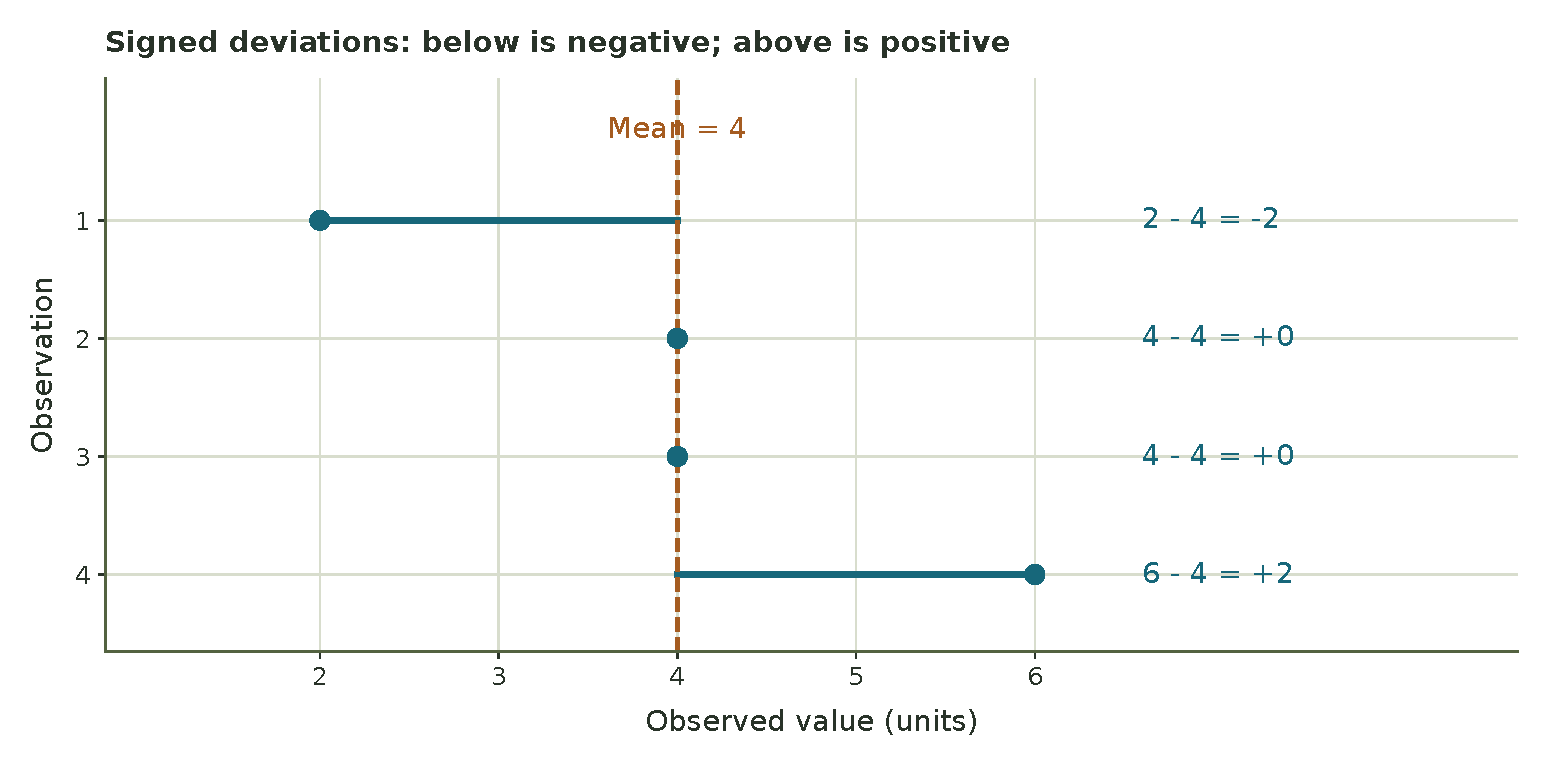
\includegraphics[width=\linewidth,height=2.9in,keepaspectratio]{../assets/week3/signed-deviations.pdf}
\captionof*{figure}{The signs locate values relative to the mean. Opposite signed deviations can cancel even when the measurements vary.}
\end{minipage}\par\medskip

For 2, 4, 4, 6, the deviations add to $-$2 + 0 + 0 + 2 = 0. The zero does not mean there is no variation. It means the mean is a balance point: the signed departures below and above it cancel.


Simply averaging those signed deviations would always give zero, apart from rounding. To describe spread, we need a calculation in which departures cannot cancel each other.


\begin{tcolorbox}[title={Pause and try 6},breakable]
For 1, 3, and 5, find the mean and the three deviations.
\end{tcolorbox}


\Needspace{6\baselineskip}\section{Sample standard deviation, one step at a time}

The \emph{sample standard deviation}, written s, describes spread around the mean using every observation. It is useful to think of it as a scale for distances from the mean. It is not calculated by averaging the ordinary distances.


Square each deviation so opposite signs cannot cancel. Add those squares. For a sample, divide by n $-$ 1 to obtain the \emph{sample variance}. Finally, take the square root to return to the original units.

\[s=\sqrt{\frac{(x_1-\bar x)^2+\cdots+(x_n-\bar x)^2}{n-1}}.\]
The compact symbol \(\sum\) sometimes replaces the long addition. It means ``add these terms.'' Work down the columns of a table before trying to do the whole formula at once.


\par\medskip{\small\renewcommand{\arraystretch}{1.35}\begin{tabularx}{\linewidth}{@{}YYY@{}}\toprule
Value x & Deviation x $-$ 4 & Squared deviation\\
\midrule
2 & $-$2 & 4\\
4 & 0 & 0\\
4 & 0 & 0\\
6 & 2 & 4\\
Total & 0 & 8\\
\bottomrule\end{tabularx}}\par\medskip

\begin{tcolorbox}[title={Complete the last two steps},breakable]

There are four observations, so n $-$ 1 = 3. The sample variance is 8/3 $\approx$ 2.67 squared units. The sample standard deviation is \(\sqrt{8/3}\approx1.63\) original units. Keep the fraction until the last step; rounding the variance too early can change the answer.


\end{tcolorbox}

\par\medskip\noindent\begin{minipage}{\linewidth}
\centering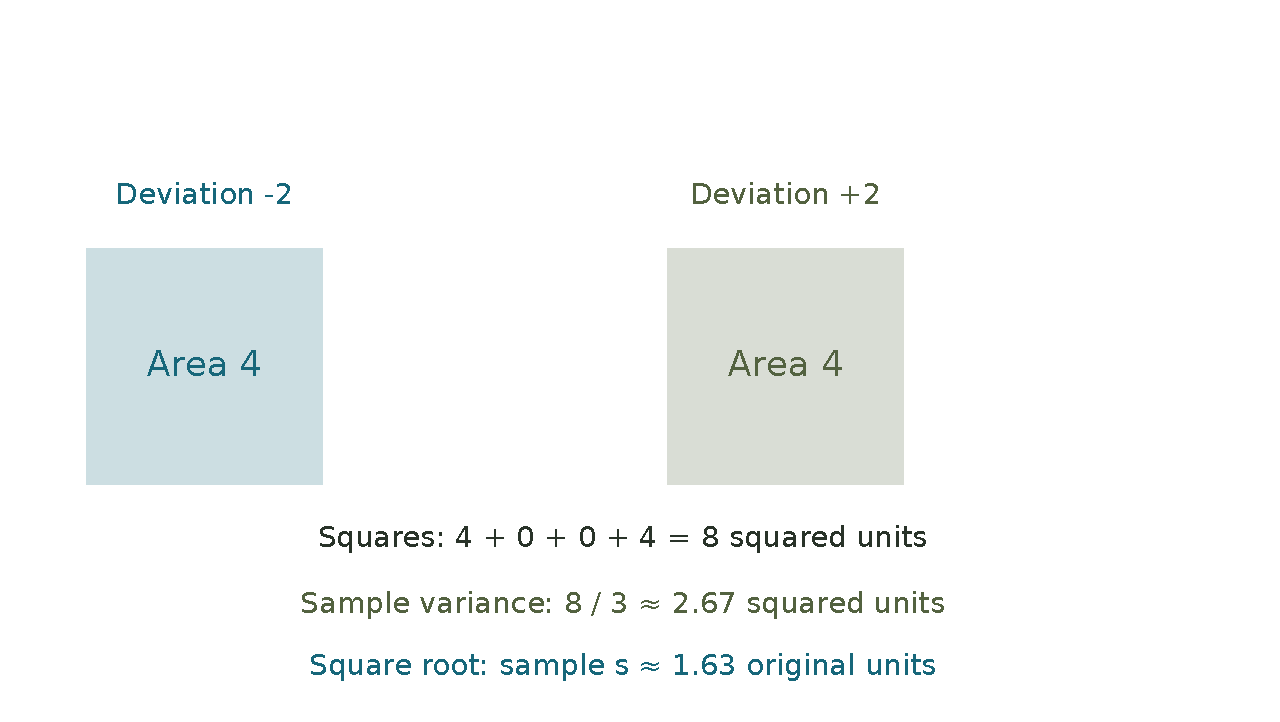
\includegraphics[width=\linewidth,height=2.65in,keepaspectratio]{../assets/week3/squares-and-units.pdf}
\captionof*{figure}{Squaring changes the units. The final square root makes standard deviation comparable with the original measurements.}
\end{minipage}\par\medskip

Why n $-$ 1? We have already used the sample to find its mean. Once that mean and all but one deviation are known, the last deviation is fixed by their sum being zero. The sample-variance rule allows for that lost freedom. Its statistical justification concerns estimating variation in a larger population; you do not need that proof to follow the calculation here.


Some calculators offer both a sample SD and a population SD. A population calculation divides by the full count when the list is the entire population being described. These assigned calculations use the \emph{sample} formula and n $-$ 1. At least two observations are needed. With two or more identical values, s = 0.


\begin{tcolorbox}[title={Pause and try 7},breakable]
For 1, 3, and 5, the squared deviations total 8. Find the sample variance and sample standard deviation.
\end{tcolorbox}


\Needspace{6\baselineskip}\section{Look at the graph as well as the summaries}

Compare centers first, then spreads, while keeping the setting and units in view. A larger standard deviation means greater spread around that mean. It does not automatically mean better performance.


\par\medskip\noindent\begin{minipage}{\linewidth}
\centering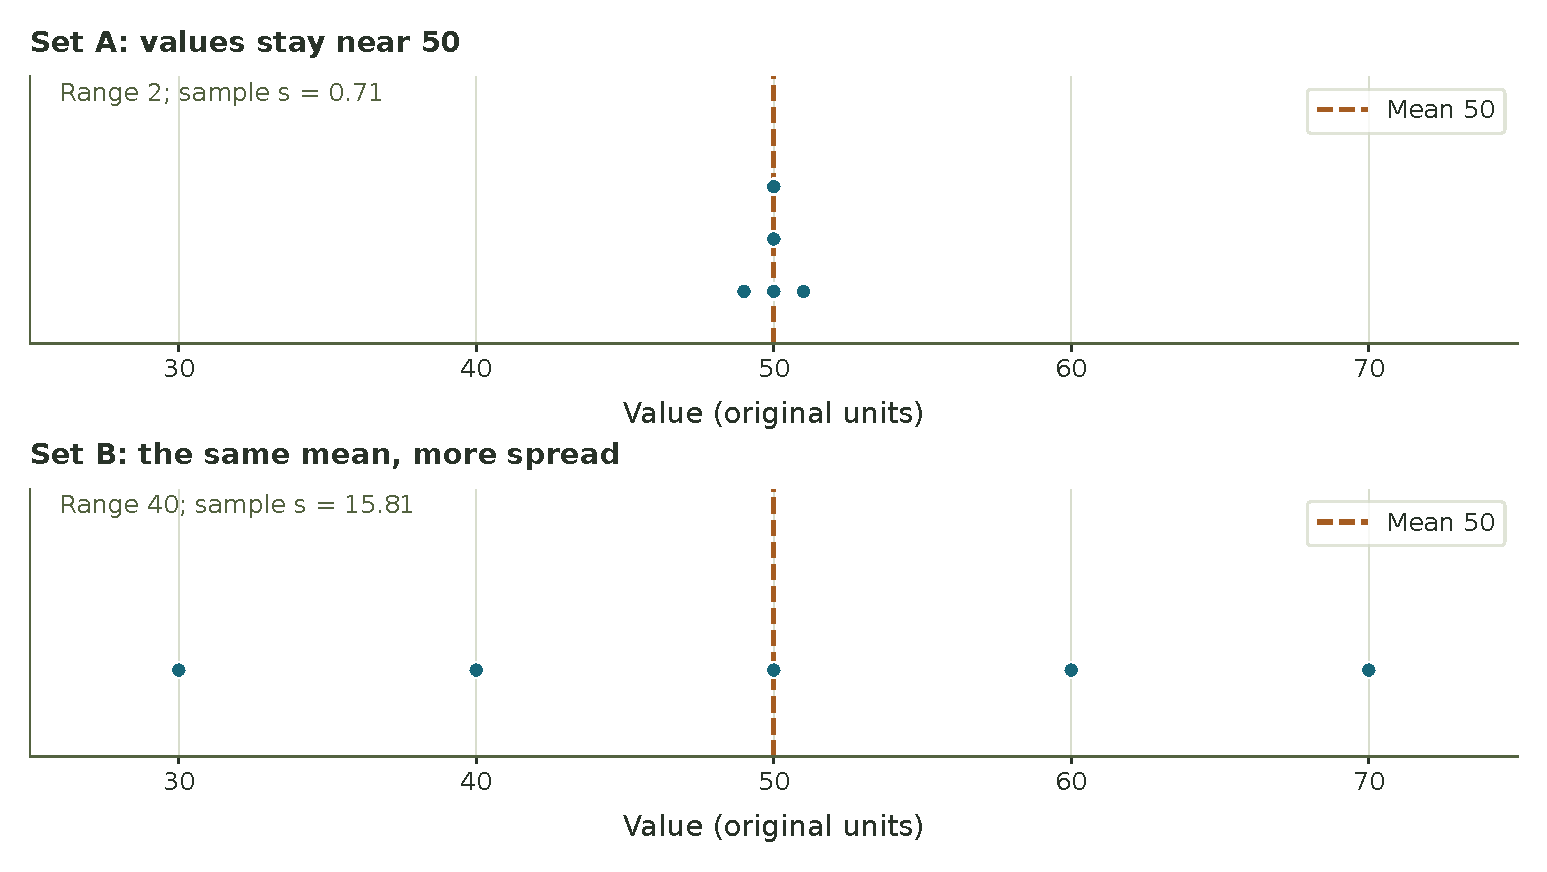
\includegraphics[width=\linewidth,height=3.0in,keepaspectratio]{../assets/week3/same-mean-spread.pdf}
\captionof*{figure}{The same axis makes the difference visible. Range and sample standard deviation both show that the second sample is more spread out.}
\end{minipage}\par\medskip

Now consider five weekly amounts: 10, 12, 13, 14, and 101 dollars. Their mean is 30 dollars; their median is 13 dollars. The mean correctly shares the full total of 150 dollars. The median better describes the middle of these particular weekly amounts.


\par\medskip\noindent\begin{minipage}{\linewidth}
\centering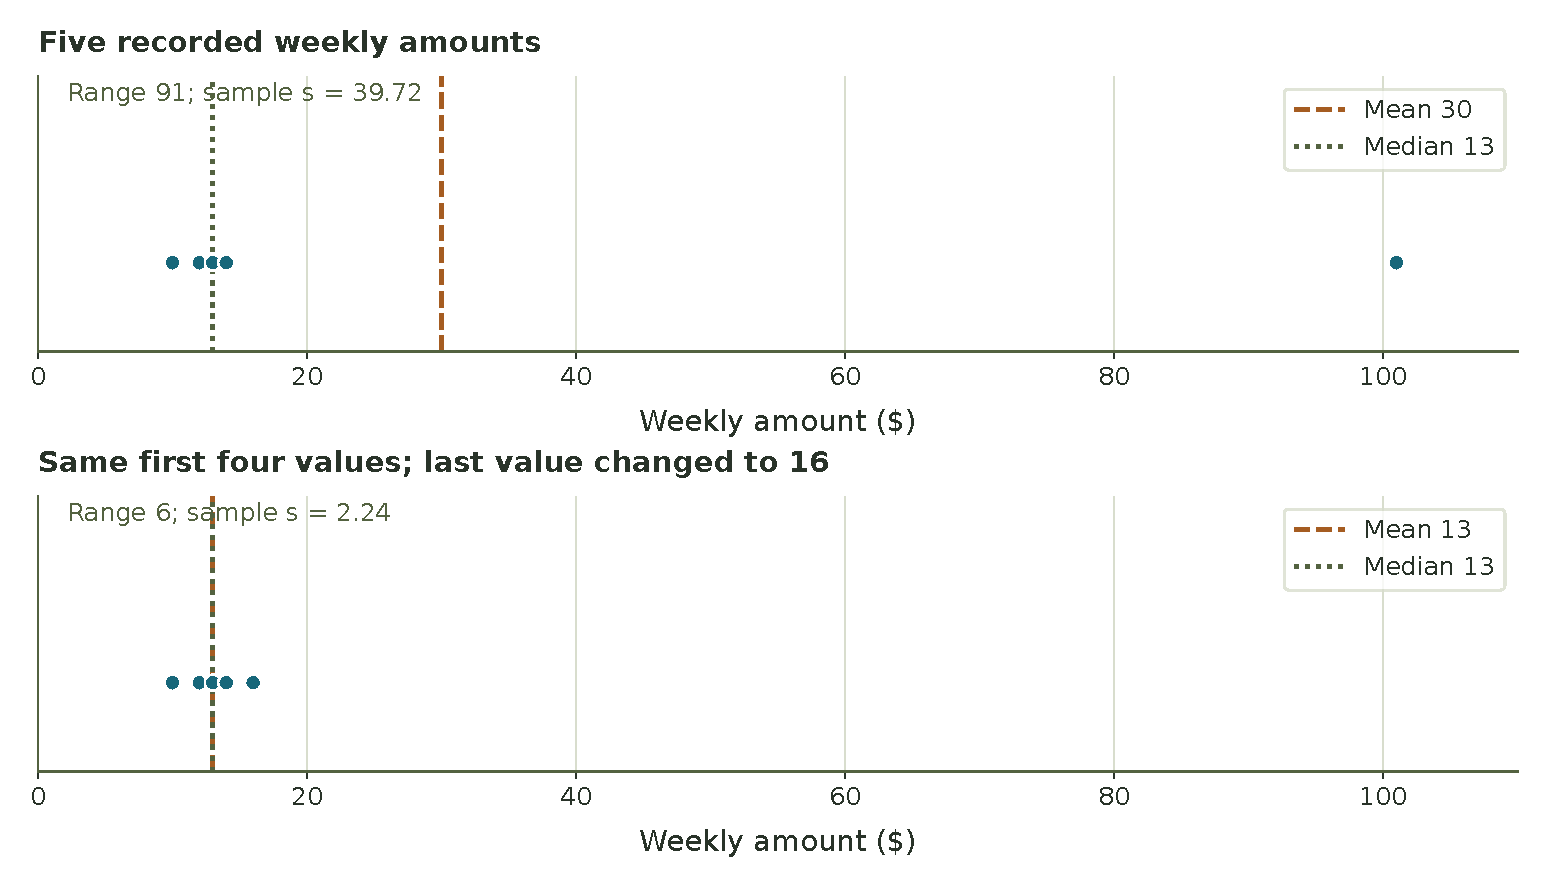
\includegraphics[width=\linewidth,height=3.1in,keepaspectratio]{../assets/week3/outlier-center.pdf}
\captionof*{figure}{An unusually distant value can strongly change the mean, range, and standard deviation. The median is often less sensitive.}
\end{minipage}\par\medskip

A value far from the others is worth investigating. It could be a recording error or a real unusual event. Comparing summaries with and without it shows its influence; it does not by itself justify deleting the observation.


The range is \emph{not} resistant to extreme values. Using a median alongside a range does not make the range resistant. For this course, calculate the requested measures and explain what each reveals. Other courses may introduce measures such as the interquartile range that focus on the middle part of the data.


Histograms group observations into intervals. A bar's height counts observations in that interval. The tallest bar identifies a most common interval, not necessarily the location of the mean or median.


\par\medskip\noindent\begin{minipage}{\linewidth}
\centering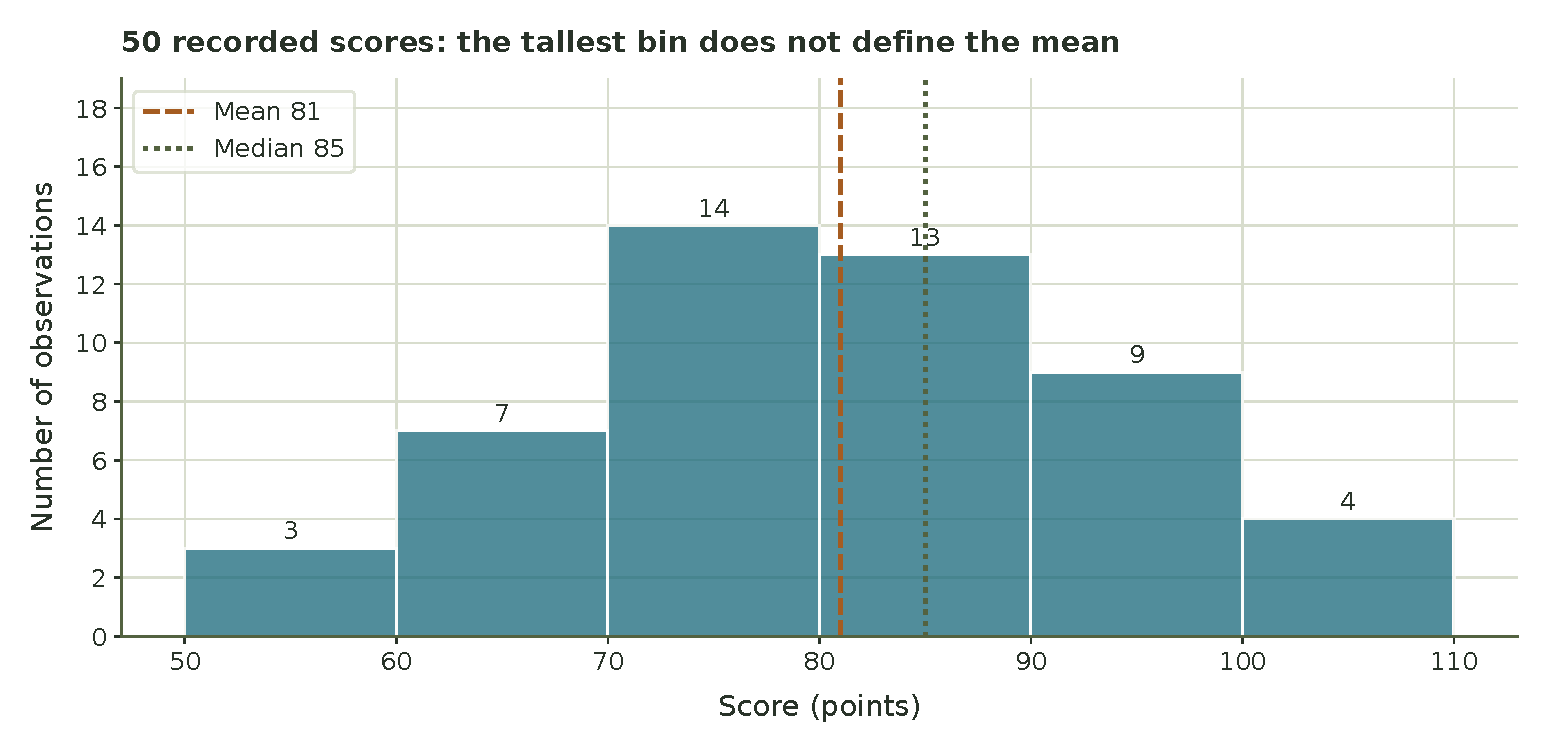
\includegraphics[width=\linewidth,height=2.65in,keepaspectratio]{../assets/week3/histogram-center.pdf}
\captionof*{figure}{Here the raw scores are 55, 65, 75, 85, 95, and 105, occurring 3, 7, 14, 13, 9, and 4 times. The tallest bin contains 28\% of the sample, not a majority.}
\end{minipage}\par\medskip

\begin{tcolorbox}[title={Pause and try 8},breakable]
If a sample has one very large value, is the range protected from its effect by reporting the median?
\end{tcolorbox}
